\section{Theory}
\label{sec:theory}

\fboxsep=1mm%padding thickness
\fboxrule=1pt%border thickness

\begin{figure*}[!ht]
	\centering
	\begin{subfigure}{0.27\linewidth}
		%  trim={<left> <lower> <right> <upper>}
        %\fcolorbox{red}{yellow}{
            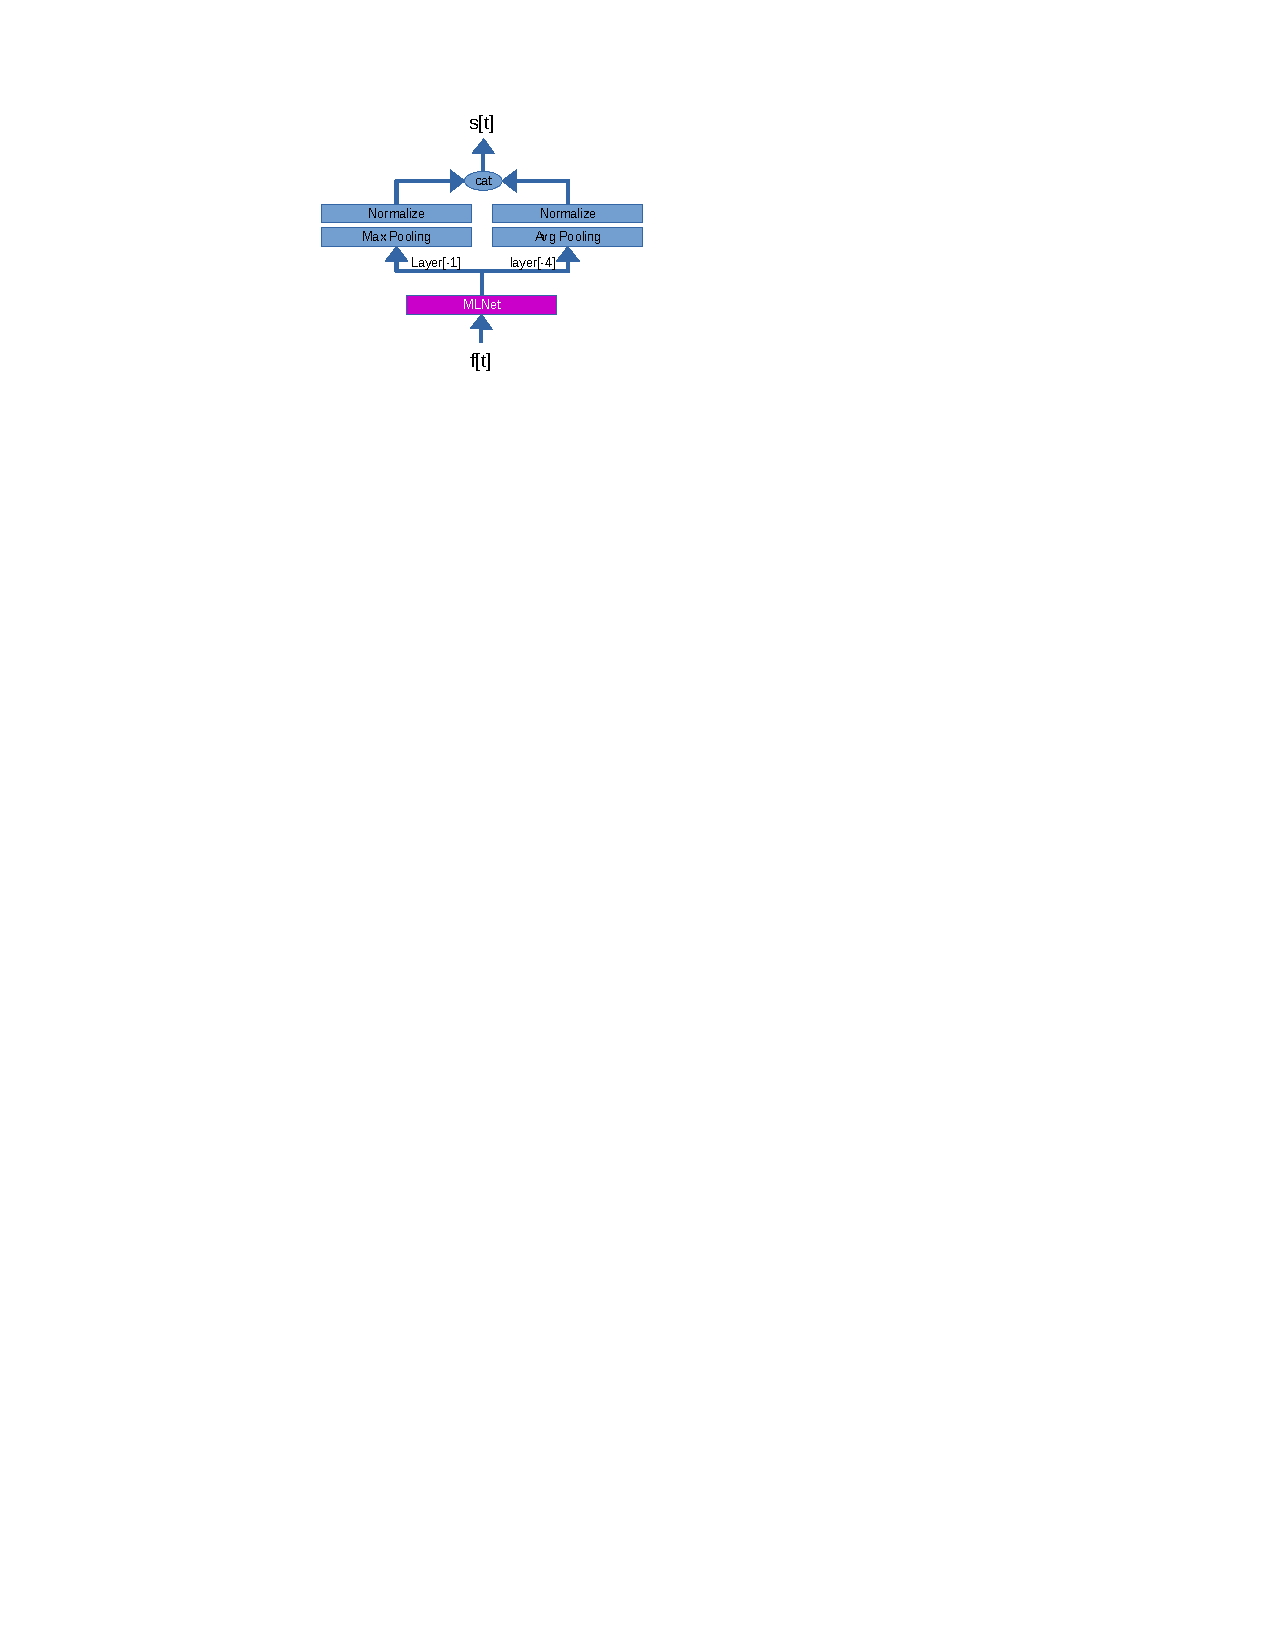
\includegraphics[trim=140 580 300 50, clip, width=1.\linewidth]{images/saliency.pdf}
        %}
        \caption{Saliency module architecture.}
        \label{fig:arch-saliency}
	\end{subfigure}
	\begin{subfigure}{0.7\linewidth}
		%  trim={<left> <lower> <right> <upper>}
        %\fcolorbox{red}{yellow}{
            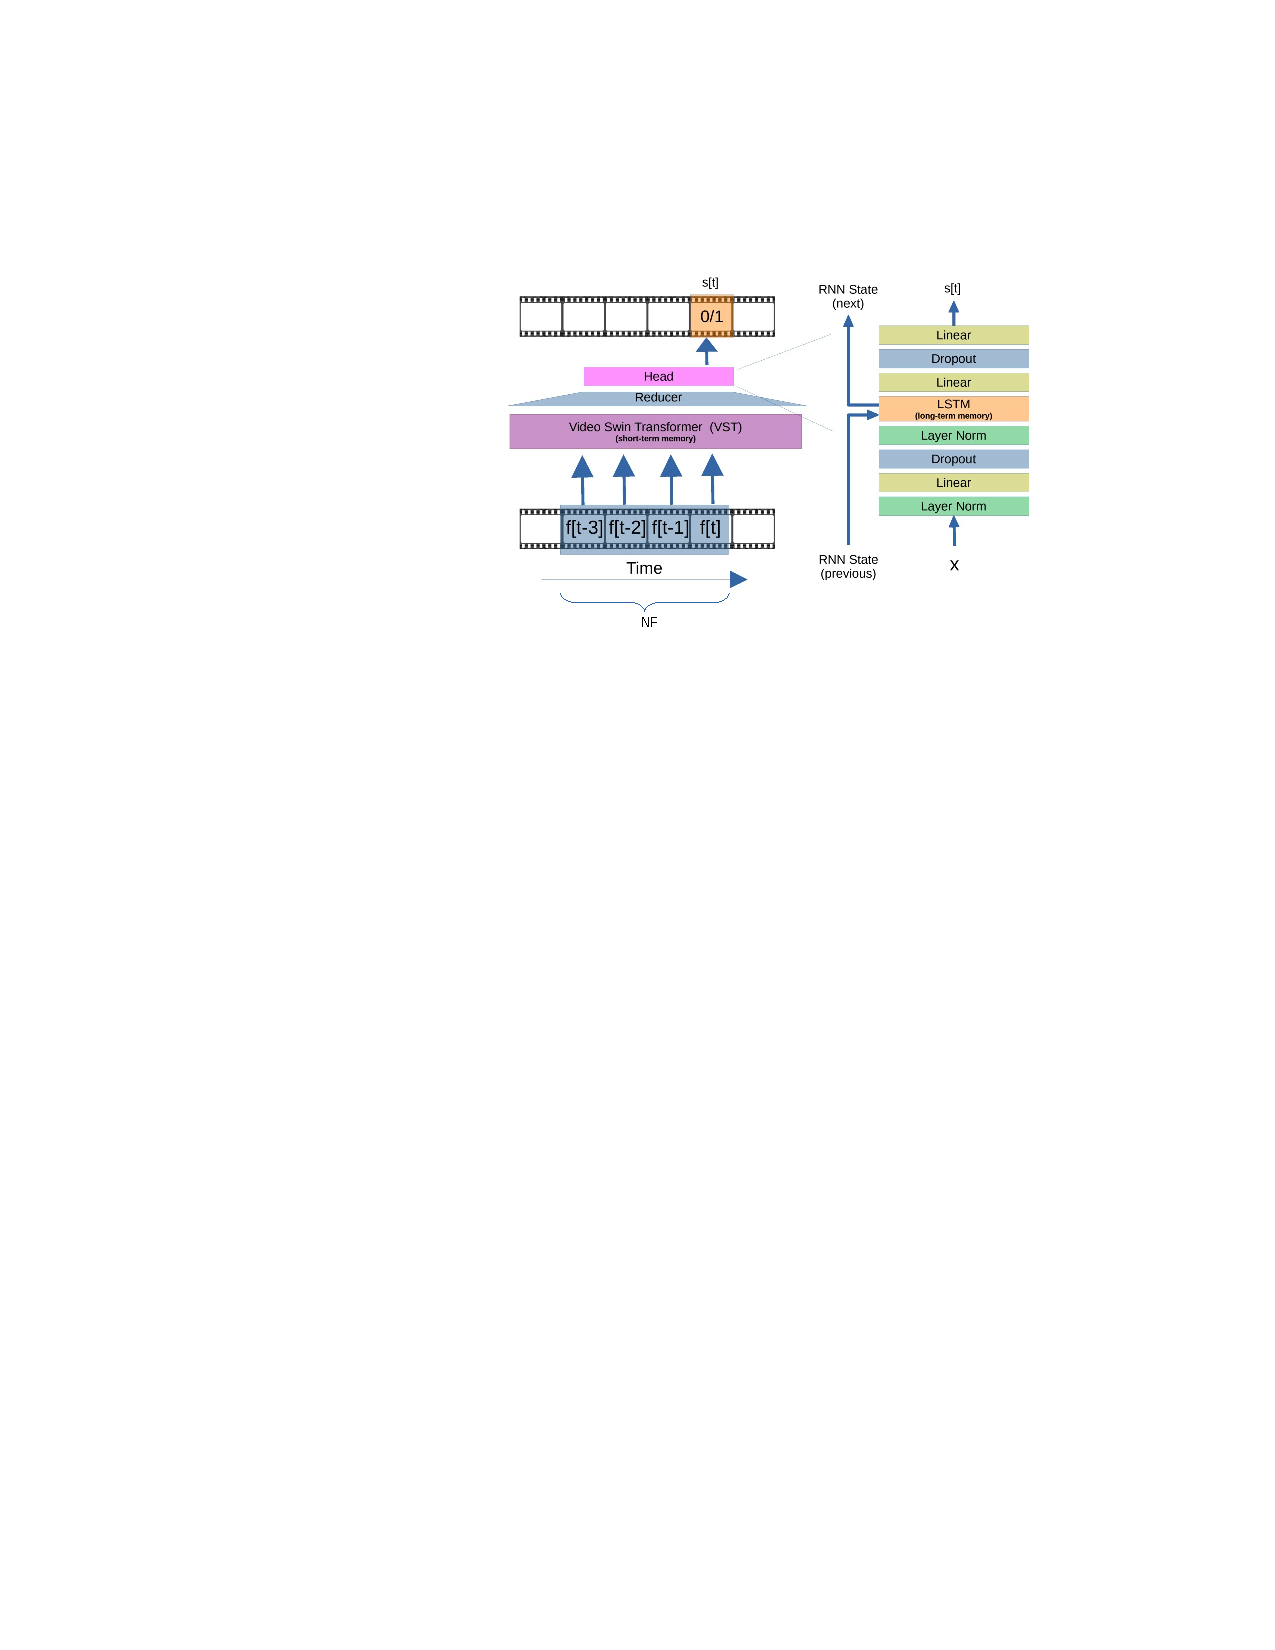
\includegraphics[trim=205 500 80 130, clip, width=1.\linewidth]{images/arch.pdf}
        %}
        % FIXME aggiungi link per immagine dei frame (copyright)
        \caption{Our online video frame anomaly detection architecture.}
		\label{fig:arch}
	\end{subfigure}
	\caption{On left the saliency module architecture more in details. On right the overall architecture. $f[t]$, $x$ are the frame at time $t$ and the output of the Reducer, respectively.}
	\label{fig:our-arch}
\end{figure*}

In this section, the overall architecture shown in Figure~\ref{fig:arch} will be explained.
The final architecture and training modality are very simple and straightforward.
The model is composed by four main blocks: a short-term memory module to encode the information related to what is happening in the present and the near past, a long-term memory module to keep track of the remote past, a saliency module to increase the relevant information about the current frame scene and the final classification module.
% TODO descrivere la nuova annotazione ??? Check motivazioni! :)

\noindent\textbf{Short-term memory}
%TODO Breve accenno su tranformer
Taking inspiration from \cite{xu2021long}, recently observed frames have been taken into account as a source of information related to the ongoing action, and past frames as a source of information on the context.
For the former, we adopted a Vision Transformer \cite{DBLP:conf/iclr/DosovitskiyB0WZ21} solution, which has become very popular in computer vision tasks, challenging the predominance of CNN architectures.
To model short-term memory, a Transformer model was chosen instead of an RNN due to its ability to process frames in parallel.
Since the task requires an online anomaly frame classification, it means the only information available are the current and the past frames.
At each step, the number of processed frames are three: the current one and the previous two frames.
The network has to take the time into consideration, as incorrect behavior is often recognizable by taking into consideration the immediate past.
In particular, the Video Swin Transformer (VST) \cite{liu_video_2022} was chosen as the base model due to its superior performance compared to a vanilla ViT \cite{DBLP:conf/iclr/DosovitskiyB0WZ21} model.
The VST model is the extension to video of the Swin Transformer \cite{liu2021Swin}, which is a general-purpose image backbone with high performance on tasks that involve detection and localization.
Originally born to carry out the task of video action classification, analyzing all the frames in one pass, it has been adapted in this work to detect anomalies on single frame at time $t_{i}$, in a near-real time fashion, considering a temporal window of the latest three frames at time $t_{i-2}$, $t_{i-1}$ and $t_{i}$.

The VST takes as input a video with size $T \times H \times W \times 3$, where $T$, $H$ e $W$ correspond to number of frames, height, width and channels RGB, respectively.
The model internally split the frames in non-overlapping 3D patches, partitioning the video in $\frac{T}{2} \times \frac{H}{4} \times \frac{W}{4}$ 3D tokens, projecting the features to an arbitrary dimension $C$.
The rest of the architecture is similar to Swin Transformer, with four stages of Video Swin Transformer block, interspersed with $2\times$ spatial downsampling in the patch merging layer.
As shown in Figure \ref{fig:arch}, the input of the VST is formed by $f[t-2]$, $f[t-1]$ and $f[t]$, which are buffered past frames at times $t-2$ and $t-1$, and the current frame at time $t$, respectively.

\noindent\textbf{Long-term memory.}
In order to not lose information from the distant past, we needed a way to keep track of it.
Because the model is working in an online fashion, this time the requirement is opposite compared to the short-term memory.
We can only update the long-term memory sequentially, when a new frame is available.
For this reason, our choice fell on an RNN module (LSTM in this specific case) instead of a Transformer.
%Its hidden state $h_t$ and cell state $c_t$ encode information about the past.
Because it doesn't need to access the past frames again, but only the latent features, the module is very efficient and lead to a limited additional computational cost.
Indeed, it condenses all its knowledge into two states: an hidden state $h_t$ and cell state $c_t$.
Since the output of the first Linear layer of the classifier head provides the summary about the three frames processed by the short-term memory model, the LSTM cells is added immediately after updating the memory states with the new information.
\vnote{specificare che le celle LSTM sono stacked qui o in experiments}

\noindent\textbf{Saliency model.}
%Determining an anomalous scene implies to evaluate the salient regions
Human capability of evaluating danger on the fly is still a matter of study by neuro-scientists.
When comparing machine to humans in the task of describing the content of an image we know that the latter perform better \cite{jiang2015salicon}.
Since we are aiming to develop a system capable of estimating danger in traffic video scenes, it is worth emulating how humans focus on important regions or objects in images through saliency estimation.
For this reason, we decided to support the model with a system that detects this information in parallel.
Taking inspiration from DRIVE \cite{bao2021drive}, we added more information about the scene present in the current frame with the help of a saliency model, used in evaluation mode.
The fixation information tells us which regions of the frame attract a person's attention, simulating what human see at first glance.
Having a saliency network trained to predict where a person's attention would be focused will most likely give us some hints in advance about hot spots where anomalous action is likely to occur. \tnote{qui stiamo attenti all'obiezione che potrebbero fare sul fatto che i posti dove siamo soliti guardare potrebbero non essere quelli dove avviene l'anomalia.}
We adopted a VGG-16-based MLNet \cite{cornia2016deep} as saliency module, pre-trained on the fixation data of the DADA-2000 \cite{fang2019dada} training set, and we frozen the parameters during the new training.
As seen in the Figure \ref{fig:arch-saliency}, we normalized and concatenated the output of MLNet last layer and the fourth last layer, to form a single saliency vector $s[t]$ of 2275 values.
Before the concatenation, the features are passed through a max pooling and average pooling, respectively.
In this way we lose some of the locality information, but we get a compact version, efficiently processed by the following fully-connected layers.

\noindent\textbf{Classification module (Head).}
After reducing the output of the VST with a Adaptive Average Pool 3D (Reducer), the classification module process it, generating the anomaly classification score for the current frame.
As shown in Figure \ref{fig:arch}, the head is composed by some Linear layers, the LSTM cells which compose the long-term memory and the branch connected with the saliency module.
For each frame at time $t$, the final output is the anomaly classification score $s_t \in [0,1]$, where $s_t=0$ means absence of anomaly and $s_t=1$ means the frame is surely anomalous.
This is trained with a weighted cross-entropy loss, giving more weight to the anomaly class, because it is spotted less frequently \tnote{scriviamo il rapporto fra le due classi: 70/30?} \vnote{TODO: contare il numero effettivo di frame anomali/normali}.

%train  dataset:  3191  video annotations found
%Normal frames found:  221429
%Anomaly frames found: 108121
%val  dataset:  1376  video annotations found
%Normal frames found:  94347
%Anomaly frames found: 46971

% copyright image frame: <a href="https://www.freepik.com/free-vector/realistic-vector-icon-film-tape-strip-with-white-square-isolated-white-cinema-concept_31096470.htm#query=video%20frame&position=31&from_view=keyword">Image by user15245033</a> on Freepik